\documentclass[dissertacao]{ppgccufscar}
\hyphenation{op-tical net-works semi-conduc-tor}

\usepackage[brazil]{babel}
\usepackage[utf8]{inputenc}
\usepackage[pdftex]{graphicx}
\usepackage{ifpdf}
\usepackage[alf]{abntcite}
\usepackage{subfig}
\usepackage{algorithm2e}
\usepackage{url}
\usepackage{enumerate}
\usepackage{indentfirst}
\setlength{\parindent}{1.5cm}


\titulo{Proxy RouteFlow Baseado em Java}
%\titulo{Proxy RouteFlow Baseado em Java Usando o Controlador Floodlight}
\autor{Fabiano Silva Mathilde}
\orientador[Orientador]{Prof. Dr. Cesar Augusto Cavalheiro Marcondes}
\coorientador[Coorientador]{Dr. Christian Esteve Rothenberg}
\areaconcentracao{Sistemas Distribuídos e Redes}
\data{Janeiro/2013}


\begin{document} 

\capa
\folhaderosto
\dataaprovacao{29}{Janeiro}{2013}
\begin{folhadeaprovacao}
%\examinador{Prof. Dr.Hermes Senger }{DC - UFSCar}
%\examinador{Prof. Dr. Magnos Martinello }{UFES}
\end{folhadeaprovacao}

\begin{resumo}

Nos últimos anos o protocolo \textit{OpenFlow} 
vem aumentando a visibilidade das tecnologias 
de redes definidas por software, fazendo com 
que um número cada vez maior de pesquisadores 
e desenvolvedores o adotem como principal
 ferramenta para simulações ou aplicações em
 ambientes reais. O projeto comunitário
 \textit{RouteFlow}, liderado pela Fundação 
\textit{CPqD}, propõe uma plataforma de 
roteamento IP definido por software (do
 termo em inglês, \textit{software-defined networking}) 
baseado no protocolo \textit{OpenFlow}, que permite 
uma separação efetiva do plano de controle do plano 
de encaminhamento dos equipamentos de rede. O 
fato do sistema ter sido criado com o código totalmente
 aberto fez com que o número de usuários aumenta-se 
consideravelmente incentivando a equipe de 
desenvolvedores a atualizá-la constantemente 
para agregar cada vez mais ferramentas e 
tecnologias. O \textit{RouteFlow} faz a 
manipulação do protocolo \textit{OpenFlow} 
utilizando os softwares de controle mais famosos 
da literatura, o \textit{NOX}, criado totalmente 
em \textit{C++} e o \textit{POX}, criado 
totalmente em \textit{Python}. Para aumentar a 
capacidade do \textit{RouteFlow} o trabalho em 
questão descreve a adição de suporte à um novo 
software de controle, o \textit{Floodlight}, sendo 
criado totalmente em \textit{Java}. Sendo assim 
o \textit{RouteFlow} ganhará suporte a mais uma
 tecnologia mantendo-se sempre na vanguarda
 das tecnologias de redes definidas por software.     

\palavraschave{Redes Definidas por Software}
\end{resumo}

\begin{abstract}

In the last years the \textit{OpenFlow} 
protocol has increased the visibility of the software
 defined network technologies, causing a growing 
number of researchers and developers to adopt it as 
the main tool for simulations or applications in real 
environments. The \textit{RouteFlow} community 
project, led by CPqD Foundation, proposes a platform
 defined by IP routing software based on 
the \textit{OpenFlow} protocol, which allows 
effective separation of the control plane of routing
 equipment plan network. The fact that the system
 has been created with fully open source has caused
 the number of users increases considerably encouraging
 the development team to update it constantly adding 
more and more tools and technologies. 
The \textit{RouteFlow} manipulate  the 
\textit{OpenFlow} protocol using the most famous 
controllers of the literature, \textit{NOX}, created 
entirely in \textit{C++} and \textit{POX}, created 
entirely in Python. To increase the capacity of 
the \textit{RouteFlow}, this work describes the 
addiction of the support for a new controller, 
\textit{Floodlight}, being created entirely in 
\textit{Java}. Thus the \textit{RouteFlow} win 
support more technology always staying at the
 forefront of the software defined network technologies.

\keywords{Software Defined Network}
\end{abstract}

\listoffigures
\listoftables

%% defina aqui o seu glossario
\acronym{ISP}{\textit{Internet Service Provider}}
\acronym{IP}{\textit{Internet Protocol}}
\acronym{UDP}{\textit{User Datagram Protocol}}
\acronym{TCP}{\textit{Transmission Control Protocol}}
\acronym{OF}{\textit{OpenFlow}}
\acronym{ARP}{\textit{Address Resolution Protocol}}
\acronym{MPLS}{\textit{Multiprotocol Label Switching}}
\acronym{IPC}{\textit{Inter-Process Communication}}
\acronym{REST}{\textit{Representational State Transfer}}
\acronym{OSPF}{\textit{Open Shortest Path First}}
\acronym{BGP}{\textit{Border Gateway Protocol}}
\acronym{RIP}{\textit{Routing Information Protocol}}
\acronym{JSON}{\textit{JavaScript Object Notation}}
\acronym{API}{\textit{Application Programming Interface}}
\listofacronyms

%% sumario
\tableofcontents

\chapter{Introdução}

\section{Objetivo do Trabalho}
O trabalho tem como objetivo principal agregar um nova funcionalidade ao \textit{RouteFlow}. A funcionalidade será o suporte nativo ao controlador \textit{Floodlight}. Os controladores são usados pelo \textit{RouteFlow} como uma interface de comunicação entre os softwares de roteamento e os switches \textit{Openflow}. Cada controlador possui certas características juntamente com recursos exclusivos e com isso esperá-se que o \textit{RouteFlow} agregue as melhores ferramentas disponíveis no controlador \textit{Floodlight}.

\section{Contribuições}
Como principal contribuição do trabalho podemos citar a integração que haverá entre o \textit{RouteFlow} e a comunidade de usuários do controlador \textit{Floodlight}. A comunidade poderá realizar simulações ou até experimentos em ambientes reais contribuindo ainda mais com o avanço do \textit{RouteFlow}. Outra contribuição importante que pode ser citada é a absorção pelo  \textit{RouteFlow} das melhores ferramentas providas pelo \textit{Floodlight}, tornando-o cada vez mais completo.

\chapter{Redes Definidas por Software}

\section{Definição Geral} As Redes Definidas
por Software (Software Defined Networks, ou SDN) constituem
um novo paradigma para o desenvolvimento de pesquisas em
redes de computadores que vem ganhando a atenção de grande
parte da comunidade acadêmica e da industria da área de
redes. Fazendo um balanço geral da situação que encontramos
hoje, podemos dizer que é um pouco complexa: é possível afirmar
que a área de redes fez um sucesso estrondoso, já que hoje a
tecnologia de redes de computadores permeia todos os níveis
da sociedade. Grande parte das atividades da sociedade de
alguma forma passa por uma ou mais redes de computadores.

Mas tamanho sucesso trouxe consigo um problema para a comunidade
de pesquisa. Como grande parte da sociedade depende hoje da
internet em suas atividades diárias e as tecnologias de rede
se tornaram de fácil acesso, a estabilidade se tornou uma
característica fundamental das redes de computadores. Isso
significa que pesquisas com novas tecnologias e protocolos
já não são mais possíveis em redes de larga escala, como a
Internet, devido ao risco de interrupção ou instabilidade
dos serviços essenciais. Outro problema encontrado pelos
pesquisadores é o fato de que a larga utilização de
tecnologias já desenvolvidas inviabiliza a inserção de
qualquer tecnologia que exija a inserção de novos
equipamentos de hardware.

Mesmo pesquisadores trabalhando em redes experimentais sofrem
para justificar a adoção em larga escala das tecnologias
desenvolvidas nesses ambientes. O potencial de instabilidade
ou ruptura de tais avanços se torna um forte argumento
contra sua adoção.

Esses problemas citados acima só ocorrem pelo fato de que redes
de computadores em geral e a rede mundial (a Internet)
atingiram um nível de amadurecimento que as tornaram pouco 
flexíveis.
Para tentar melhorar essa situação, a comunidade de pesquisa
em redes de computadores tem investido em iniciativas que
levam ao desenvolvimento de redes com maiores 
recursos de programação, de forma que as novas tecnologias
possam ser inseridas na rede de forma gradual. Exemplos de
iniciativas desse tipo são as propostas de redes ativas
\textit{(active networks)} [Tennenhouse e Wetherall 2007],
de \textit{testbeds} como o PlanetLab [Peterson e Roscoe 2006]
e, mais recentemente, do GENI [Turner 2006, Elliott e Falk
2009]. Redes ativas, apesar de terem grande potencial,
tiveram pouca aceitação pela necessidade de alteração dos
elementos de rede para permitir que se tornassem programáveis. As iniciativas 
mais recentes, como o PlanetLab e o GENI, apostam na adoção
de recursos de virtualização para facilitar a transição para
novas tecnologias. Apesar de serem consideradas de
grande potencial ao longo prazo, tais iniciativas ainda
enfrentam desafios em questões como garantir o desempenho
exigido pelas aplicações largamente utilizadas hoje
utilizando-se tais elementos de rede virtualizados.

Uma outra forma de abordar o problema, a fim de oferecer
um caminho de menor impacto e que possa ser implementado 
em prazos mais curtos e com bom desempenho, consiste
em estender o hardware de encaminhamento de pacotes
de forma mais restrita. Considerando-se que a operação 
que precisa de alto desempenho nos elementos de comutação
atual é o encaminhamento de pacotes, algumas iniciativas
propõem manter essa operação pouco alterada, para manter 
a viabilidade de desenvolvimento de hardware de alto
desempenho, mas com uma possibilidade de maior controle 
por parte dos administradores de rede. Essa proposta se inspira 
em uma tecnologia já largamente adotada, o chaveamento
(encaminhamento) baseado em rótulos programáveis, 
popularizado pelo MPLS \textit{(Multi-Protocol Label
 Switching)} [Davie e Farrel 2008, Kempf et al. 2001].

Com o MPLS, o controle fino sobre o tráfego de rede se torna 
possível ao se atribuir a cada pacote um rótulo \textit{(label)}
que determina como o mesmo será tratado pelos elementos
de rede. Explorando esse recurso, administradores de rede podem
exercer controle diferenciado sobre cada tipo de tráfego de rede,
assumindo que os mesmos possam ser identificados para
receberem os rótulos apropriados. Com base nessa observação,
uma ideia trabalhada por diversos pesquisadores é a manutenção 
de um hardware de encaminhamento de alto desempenho, com
a possibilidade de permitir que os administradores de redes (ou 
os desenvolvedores de aplicações para a rede) determinem como 
os fluxos irão ser rotulados e encaminhados.

A iniciativa mais bem sucedida nesse sentido foi, sem dúvida,
definição da interface e do protocolo OpenFlow [McKeown et al.
2008]. Com o OpenFlow, os elementos de encaminhamento 
oferecem uma interface de programação simples que lhes
permite estender o acesso e controle da tabela de consulta 
utilizada pelo hardware para determinar o próximo passo de 
cada pacote recebido. Dessa forma, o encaminhamento continua 
sendo eficiente, pois a consulta à tabela de encaminhamento 
continua sendo tarefa do hardware, mas a decisão sobre 
como cada pacote deve ser processado pode ser transferida
para um nível superior, onde diferentes funcionalidades 
podem ser implementadas. Essa estrutura permite que a rede
seja controlada de forma extensível através de aplicações,
expressas em software. A esse novo paradigma, deu-se o 
nome de Redes Definidas por Software, ou \textit{Software
Defined Networks} (SDN).

Do ponto de vista histórico, as Redes Definidas por 
Software têm sua origem na definição
da arquitetura de redes \textit{Ethane}, que definia uma forma
de se implementar políticas de controle de acesso de forma 
distribuída, a partir de um mecanismo de supervisão centralizado
[Casado et al. 2009]. Naquela arquitetura, cada elemento de 
rede deveria consultar o elemento supervisor ao identificar um
novo fluxo. O supervisor consultaria um grupo de políticas 
globais para decidir, com base nas características de cada
fluxo, como o elemento de encaminhamento deveria 
tratá-lo. Essa decisão seria comunicada ao comutador na 
forma de programação de uma entrada em sua tabela de
encaminhamento com uma regra adequada para o novo fluxo (
que poderia, inclusive, ser seu descarte). Esse modelo foi
posteriormente formalizado por alguns autores na forma da 
arquitetura \textit{OpenFlow}.

\section{Introdução ao Protocolo \textit{OpenFlow}}

O \textit{OpenFlow} foi proposto pela Universidade de
Stanford para atender à demanda de validação de novas
propostas de arquiteturas e protocolos de rede (incluindo as
abordagens \textit{clean slate}) sobre equipamentos
comerciais. É definido como uma padrão aberto para Redes
Definidas por Software que tem como principal objetivo que 
se utilize equipamentos comerciais para pesquisa e 
experimentação de novos protocolos de rede, em paralelo
com a operação normal das redes. Isso é conseguido com a 
definição de uma interface de programação que permite 
ao desenvolvedor controlar diretamente os elementos de 
encaminhamento de pacotes presentes no dispositivo. Com o 
\textit{OpenFlow}, pesquisadores podem utilizar equipamentos de 
rede comerciais, que normalmente possuem maior poder 
de processamento que os comutadores utilizados em 
laboratórios de pesquisa, para realizar experimentos em redes
"de produção". Isso facilita muito a transferência dos resultados
de pesquisa para a industria. 

\section{Descrição Geral do Protocolo \textit{OpenFlow}}

Uma característica básica da arquitetura do padrão \textit{OpenFlow} 
é a separação clara entre os planos de dados e controle em
elementos de chaveamento. O plano de dados cuida do 
encaminhamento de pacotes com base em regras simples (chamadas de ações 
na terminologia \textit{OpenFlow}) associadas
a cada entrada da tabela de encaminhamento do comutador 
de pacotes (podendo ser um \textit{switch}, um roteador 
ou até mesmo um ponto de acesso sem fio).
Essas regras, definidas pelo padrão, incluem (\textit{i}) 
encaminhar o pacote para uma porta especifica do dispositivo,
(\textit{ii}) alterar parte de seus cabeçalhos, (\textit{iii}) 
descartá-los, ou (\textit{iv}) encaminhá-lo para inspeção 
por um controlador da rede. Em dispositivos dedicados, o plano
de dados pode ser implementado em hardware utilizando os
elementos comuns aos roteadores e \textit{switches} atuais.
Já o módulo de controle (ou controlador) pode ser um 
módulo de software implementado de forma independente em
algum ponto da rede.

A principal abstração utilizada na especificação
\textit{OpenFlow} é o conceito
de fluxo. Um fluxo é constituído pela combinação de campos
do cabeçalho do pacote a ser processado pelo dispositivo,
conforme Figura \ref{fig:cabecalhoOpenflow}. As tuplas podem
ser formadas por campos das camadas de enlace, de rede ou de
transporte, segundo o modelo \textit{TCP/IP}. Deve-se
enfatizar que a abstração da tabela de fluxos ainda está sujeita a
refinamentos, com o objetivo de oferecer uma melhor
exposição dos recursos do hardware e, nesse caso, permitir a
concatenação de várias tabelas já disponíveis, como, por
exemplo, tabelas \textit{IP/Ethernet/MPLS}. Nesse sentido, a
contribuição mais importante do paradigma do
\textit{OpenFlow} é a generalização do plano
de dados – qualquer modelo de encaminhamento de dados
baseado na tomada de decisão fundamentada em algum valor, ou
combinação de valores, dos campos de cabeçalho dos pacotes
pode ser suportado.

\begin{figure}[hb] \centering
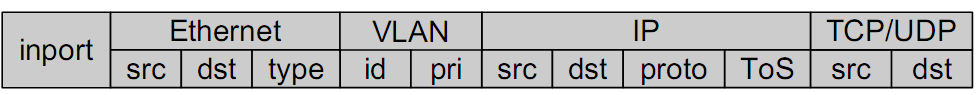
\includegraphics[width=160mm]{cabecalhoOpenflow.png}
\caption{Cabeçalho \textit{OpenFlow} para a especificação dos fluxos}
\label{fig:cabecalhoOpenflow}
\end{figure}

Um grande trunfo da arquitetura \textit{OpenFlow} é a flexibilidade 
que ela oferece para se programar de forma independente do
tratamento de cada fluxo observado, do ponto de vista de como
o mesmo deve (ou não) ser encaminhado pela rede. Basicamente,
o padrão \textit{OpenFlow} determina como um fluxo pode ser definido,
as ações que podem ser realizadas para cada pacote pertencente
a um fluxo e o protocolo de comunicação entre o comutador de 
pacotes e o controlador, utilizado para realizar alterações dessas 
definições e ações. A união de uma definição de fluxo e um
conjunto de ações forma uma entrada da tabela de fluxos 
\textit{OpenFlow} [McKeown et al. 2008].

Em um \textit{switch} \textit{OpenFlow}, cada entrada na tabela de 
fluxos pode ser implementada como um padrão de bits 
representado em uma memória TCAM (Ternary Content-
Addressable Memory). Nesse tipo de memória, bits podem
ser representados como zero, um ou "não importa" 
(\textit{don't care}), indicando que ambos os valores são
aceitáveis naquela posição. Como o padrão é programado
a partir do plano de controle, fluxos podem ser definidos da 
forma escolhida pelo controlador. A Figura \ref{fig:fluxoopenflow}
apresenta uma visão geral de uma entrada da tabela \textit{OpenFlow}.
Cada pacote que chega a um comutador \textit{OpenFlow} é comparado
com cada entrada dessa tabela; caso um casamento seja encontrado,
considera-se que o pacote pertence àquele fluxo e aplica-se
as ações relacionadas à esse fluxo. Caso um casamento não
seja encontrado, o pacote é encaminhado para o controlador 
para ser processado -- o que pode resultar na criação de uma
nova entrada para aquele fluxo. Além das ações, a arquitetura
prevê a manutenção de três contadores por fluxo: pacotes,
 \textit{bytes} trafegados e duração do fluxo. Esses contadores são 
implementados para cada entrada da tabela de fluxos e 
podem ser acessados pelo controlador através do protocolo
\textit{OpenFlow}.

\begin{figure}[hb] \centering
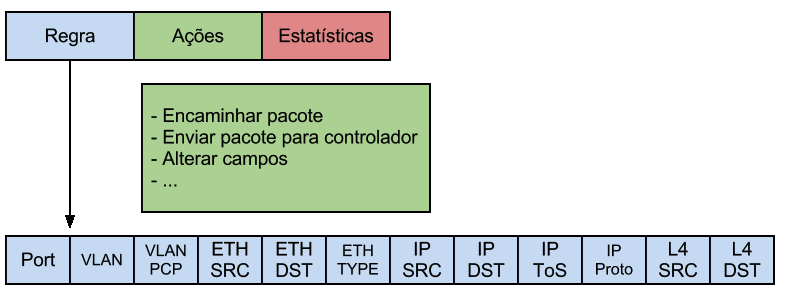
\includegraphics[width=160mm]{fluxoOpenflow.png} 
\caption{Exemplo de uma entrada na tabela de fluxos \textit{OpenFlow}.} 
\label{fig:fluxoopenflow} 
\end{figure}

Esse pequeno conjunto de regras cria diversas possibilidades,
pois muitas das funcionalidades que são implementadas 
separadamente podem ser agrupadas em um único controlador
\textit{OpenFlow}, utilizando um pequeno conjunto de regras. Alguns 
exemplos das possibilidades são apresentadas na Figura \ref{fig:exemploSwitchOpenFlow}.
As entradas representam o uso do \textit{switch} \textit{OpenFlow}
para realizar encaminhamento de pacotes na camada de enlace,
implementar um firewall e realizar encaminhamento de pacotes 
na camada de enlace utilizando redes virtuais (VLANs), respectivamente.

\begin{figure}[h] \centering
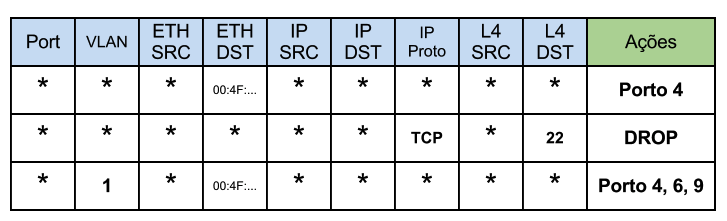
\includegraphics[width=160mm]{exemploSwitchOpenFlow.png} 
\caption{Exemplos de uso de um \textit{switch OpenFlow}.} 
\label{fig:exemploSwitchOpenFlow} 
\end{figure}

Apesar de possuir um conjunto pequeno de ações simples, 
alguns descrevem o \textit{OpenFlow} como uma analogia ao conjunto 
de instruções de um microprocessador x86 que, apesar de 
pequeno e simples, provê uma vasta gama de possibilidades 
para o desenvolvimento de aplicações. O \textit{OpenFlow} cria 
possibilidades semelhantes para o desenvolvimento de 
aplicações no contexto de redes de computadores. 

A versão atual do \textit{OpenFlow} ainda possui algumas limitações
em termos do uso padrão em circuitos ópticos e uma definição 
de fluxos que englobe protocolos que não fazem parte do 
modelo TCP/IP. No entanto, está sendo formulada uma nova
versão cujo objetivo é eliminar algumas dessas limitações.

A Figura \ref{fig:openflow} define de forma introdutória uma 
rede de computadores com o protocolo \textit{OpenFlow} habilitado. Os 
elementos comutadores podem ser de qualquer tipo, como 
comutadores convencionais, roteadores ou até mesmo pontos
de acesso sem fio. Podemos ver o elemento externo, chamado
de controlador, tomando contas das regras e ações instaladas
no hardware de rede. O controlador pode ser executado em 
qualquer equipamento com suporte à redes, como um 
servidor comum.

\begin{figure}[h] \centering
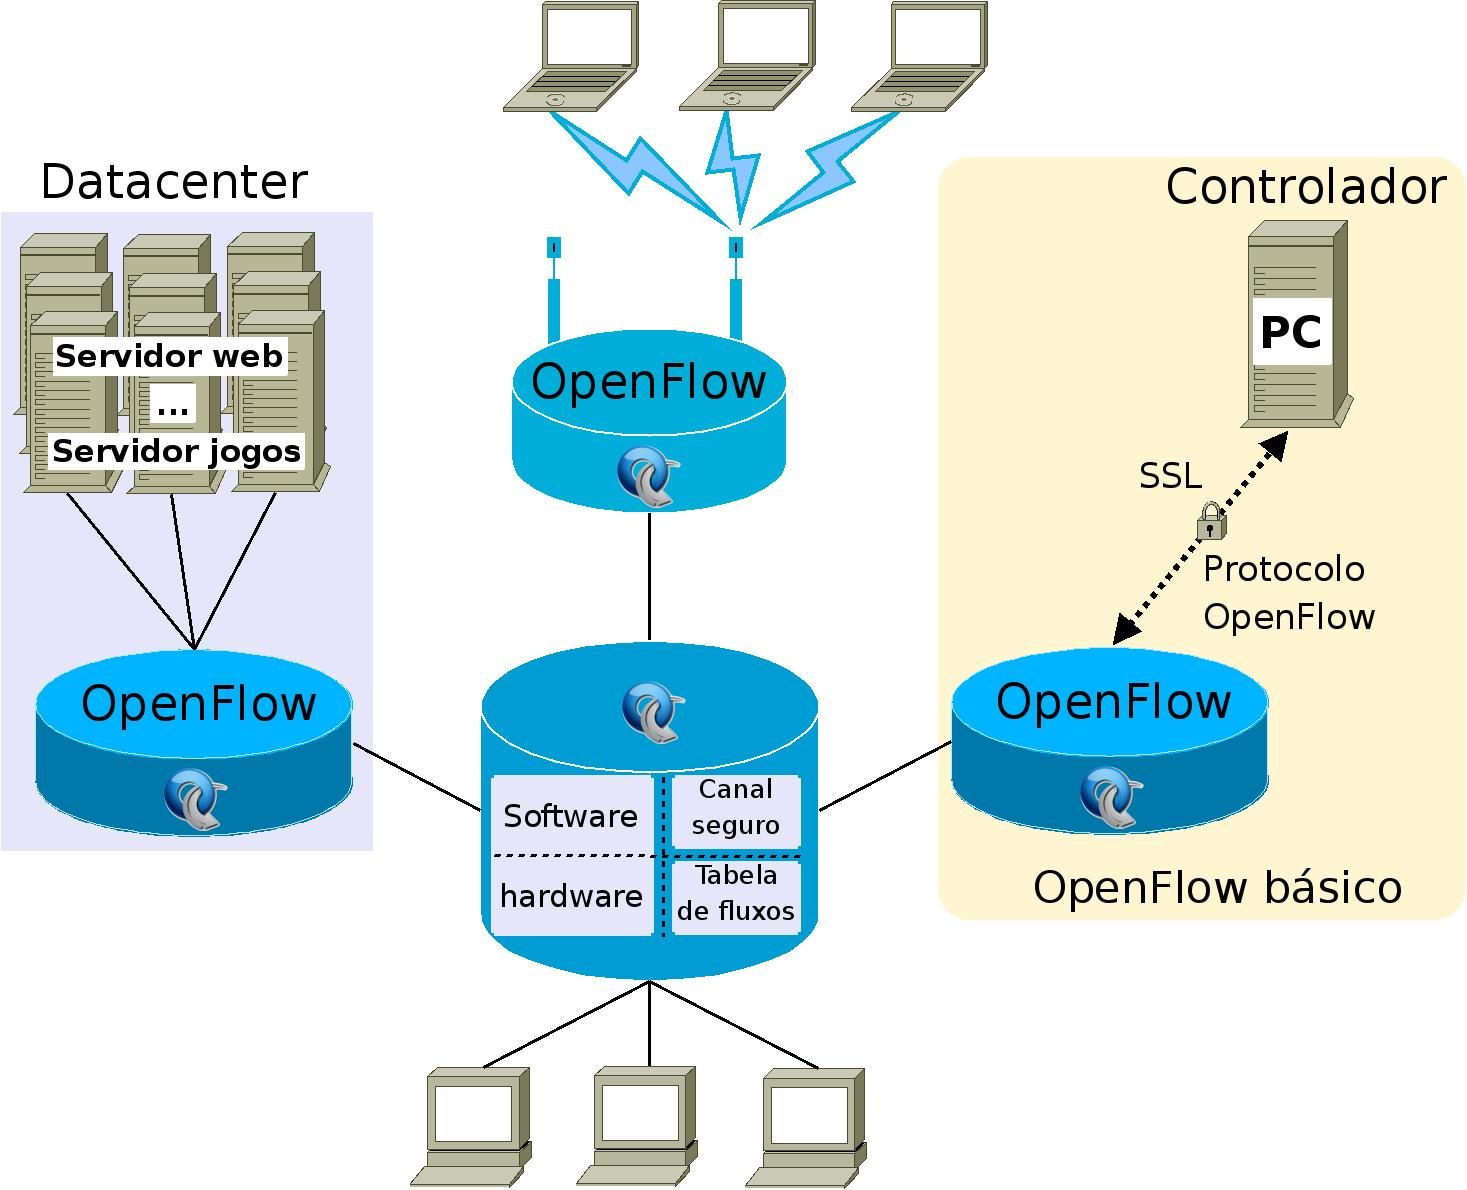
\includegraphics[width=130mm]{openflow.png} 
\caption{Rede com o protocolo \textit{OpenFlow} habilitado.} 
\label{fig:openflow} 
\end{figure}
\chapter{Arquitetura Básica do RouteFlow}

\section{Redes Definidas por Software} As Redes Definidas
por Software (Software Defined Networks, ou SDN) constituem
um novo paradigma para o desenvolvimento de pesquisas em
redes de computadores que vem ganhando a atenção de grande
parte da comunidade acadêmica e da industria da área de
redes. Fazendo um balanço geral da situação que encontramos
hoje podemos dizer que é um pouco complexa: podemos afirmar
que a área de redes fez um sucesso estrondoso, já que hoje a
tecnologia de redes de computadores permeia todos os níveis
da sociedade. Grande parte das atividades da sociedade de
alguma forma passa por uma ou mais redes de computadores.

Tamanho sucesso trouxe consigo um problema para a comunidade
de pesquisa. Como grande parte da sociedade depende hoje da
internet em suas atividades diárias e tecnologias de acesso
se tornaram de fácil acesso a estabilidade se tornou uma
característica fundamental das redes de computadores. Isso
significa que pesquisas com novas tecnologias e protocolos
já não são mais possíveis em redes de larga escala, como a
internet, devido ao risco de interrupção ou instabilidade
dos serviços essenciais. Outro problema encontrado pelos
pesquisadores é o fato de que a larga utilização de
tecnologias já desenvolvidas inviabiliza a inserção de
qualquer tecnologia que exija a inserção de novos
equipamentos de hardware.

Mesmo pesquisadores trabalhando em redes experimental sofrem
para justificar a adoção em larga escala das tecnologias
desenvolvidas nesses ambientes. O potencial de instabilidade
ou ruptura de tais avanços se torna um forte argumento
contra sua adoção.

Esses problemas citados acima só ocorrem pelo fato das redes
de computadores em geral e a rede mundial (a Internet)
atingiram um nível de amadurecimento que as tornaram pouco 
flexíveis.
Para tentar melhorar essa situação, a comunidade de pesquisa
em redes de computadores tem investido em iniciativas que
levam ao desenvolvimento de redes com maiores 
recursos de programação, de forma que as novas tecnologias
possam ser inseridas na rede de forma gradual. Exemplos de
iniciativas desse tipo são as propostas de redes ativas
\textit{(active networks)} [Tennenhouse e Wetherall 2007],
de \textit{testbeds} como o PlanetLab [Peterson e Roscoe 2006]
e, mais recentemente, do GENI [Turner 2006, Elliott e Falk
2009]. Redes ativas, apesar de terem grande potencial,
tiveram pouca aceitação pela necessidade de alteração dos
elementos de rede para permitir que se tornassem programáveis. As iniciativas 
mais recentes, como o PlanetLab e o GENI, apostam na adoção
de recursos de virtualização para facilitar a transição para
novas tecnologias. Apenas de serem consideradas de
grande potencial ao longo prazo, tais iniciativas ainda
enfrentam desafios em questões como garantir o desempenho
exigido pelas aplicações largamente utilizadas hoje
utilizando-se tais elementos de rede virtualizados.

Uma outra forma de abordar o problema, a fim de oferecer
um caminho de menor impacto e que possa ser implementado 
em prazos mais curtos e com bom desempenho, consiste
em estender o hardware de encaminhamento de pacotes
de forma mais restrita. Considerando-se que a operação 
que precisa de alto desempenho nos elementos de comutação
atual é o encaminhamento de pacotes, algumas iniciativas
propõem manter essa operação pouco alterada, para manter 
a viabilidade de desenvolvimento de hardware de alto
desempenho, mas com uma possibilidade de maior controle 
por parte do administrador de rede. Essa proposta se inspira 
em uma tecnologia já largamente adotada, o chaveamento
(encaminhamento) baseado em rótulos programáveis, 
popularizado pelo MLPS \textit{(Multi-protocol Label
 Switching)} [Davie e Farrel 2008, Kempf et al. 2001].

Com o MPLS, o controle fino sobre o tráfego de rede se torna 
possível ao se atribuir a cada pacote um rótulo \textit{(label)}
que determina como o mesmo será tratado pelos elementos
de rede. Explorando esse recurso, administradores de rede podem
exercer controle diferenciado sobre cada tipo de tráfego de rede,
assumindo que os mesmos possam ser identificados para
receberem os rótulos apropriados. Com base nessa observação,
uma ideia trabalhada por diversos pesquisadores é a manutenção 
de um hardware de encaminhamento de alto desempenho, com
a possibilidade de permitir que o administrador de rede (ou 
o desenvolvedor de aplicações para a rede) determine como 
os fluxos irão ser rotulados e encaminhados.

A iniciativa mais bem sucedida nesse sentido foi, sem dúvida,
definição da interface e do protocolo OpenFlow [McKeown et al.
2008]. Com o OpenFlow, os elementos de encaminhamento 
oferecem uma interface de programação simples que lhes
permite estender o acesso e controle da tabela de consulta 
utilizada pelo hardware para determinar o próximo passo de 
cada pacote recebido. Dessa forma, o encaminhamento continua 
sendo eficiente, pois a consulta à tabela de encaminhamento 
continua sendo tarefa do hardware, mas a decisão sobre 
como cada pacote deve ser processado pode ser transferida
para um nível superior, onde diferentes funcionalidades 
podem ser implementadas. Essa estrutura permite que a rede
seja controlada de forma extensível através de aplicações,
expressas em software. A esse novo paradigma, deu-se o 
nome de Redes Definidas por Software, ou \textit{Software
Defined Networks} (SDN).

Do ponto de vista histórico, SDNs têm sua origem na definição
da arquitetura de redes \textit{Ethane}. que definia uma forma
de se implementar políticas de controle de acesso de forma 
distribuída, a partir de um mecanismo de supervisão centralizado
[Casado et al. 2009]. Naquela arquitetura, cada elemento de 
rede deveria consultar o elemento supervisor ao identificar um
novo fluxo. O supervisor consultaria um grupo de políticas 
globais para decidir, com base nas características de cada
fluxo, como o elemento de encaminhamento que deveria 
tratá-lo. Essa decisão seria comunicada ao comutador na 
forma de programação de uma entrada em sua tabela de
encaminhamento com uma regra adequada para o novo fluxo (
que poderia, inclusive, ser seu descarte). Esse modelo foi
posteriormente formalizado por alguns autores na forma da 
arquitetura OpenFlow.

\section{Descrição do Protocolo OpenFlow}

O \textit{OpenFlow} foi proposto pela Universidade de
Stanford para atender à demanda de validação de novas
propostas de arquiteturas e protocolos de rede (incluindo as
abordagens \textit{clean slate}) sobre equipamentos
comerciais. É definido como uma padrão aberto para Redes
Definidas por Software que tem como principal objetivo que 
se utilize equipamentos de redes comerciais para pesquisa e 
experimentação de novos protocolos de rede, em paralelo
com a operação normal das redes. Isso é conseguido com a 
definição de uma interface de programação que permite 
ao desenvolvedor controlar diretamente os elementos de 
encaminhamento de pacotes presentes no dispositivo. Com o 
OpenFlow, pesquisadores podem utilizar equipamentos de 
rede comerciais, que normalmente possuem maior poder 
de processamento que os comutadores utilizados em 
laboratórios de pesquisa, para realizar experimentos em redes
"de produção". Isso facilita muito a transferência dos resultados
de pesquisa para a industria. 

Uma característica básica da arquitetura do padrão OpenFlow 
é a separação clara entre os planos de dados e controle em
elementos de chaveamento. O plano de dados cuida do 
encaminhamento de pacotes com base em regras simples (
chamadas de ações na terminologia OpenFlow) associadas
a cada entrada da tabela de encaminhamento do comutador 
de pacotes (podendo ser um \textit{switch} ou um roteador).
Essas regras, definidas pelo padrão, incluem (\textit{i}) 
encaminhar o pacote para uma porta especifica do dispositivo,
(\textit{ii}) alterar parte de seus cabeçalhos, (\textit{iii}) 
descartá-los, ou (\textit{iv}) encaminhá-lo para inspeção 
por um controlador da rede. Em dispositivos dedicados, o plano
de dados pode ser implementado em hardware utilizando os
elementos comuns aos roteadores e \textit{switches} atuais.
Já o módulo de controle permite ao controlador pode ser um 
módulo de software implementado de forma independente em
algum ponto da rede.

A principal abstração utilizada na especificação
\textit{OpenFlow} é o conceito
de fluxo. Um fluxo é constituído pela combinação de campos
do cabeçalho do pacote a ser processado pelo dispositivo,
conforme Figura \ref{fig:cabecalhoOpenflow}. As tuplas podem
ser formadas por campos das camadas de enlace, de rede ou de
transporte, segundo o modelo \textit{TCP/IP}. Deve-se
enfatizar que a abstração da tabela de fluxos ainda está sujeita a
refinamentos, com o objetivo de oferecer uma melhor
exposição dos recursos do hardware e, nesse caso, permitir a
concatenação de várias tabelas já disponíveis, como, por
exemplo, tabelas \textit{IP/Ethernet/MPLS}. Nesse sentido, a
contribuição mais importante do paradigma do
\textit{OpenFlow} é a generalização do plano
de dados – qualquer modelo de encaminhamento de dados
baseado na tomada de decisão fundamentada em algum valor, ou
combinação de valores, dos campos de cabeçalho dos pacotes
pode ser suportado.

Um grande trunfo da arquitetura OpenFlow é a flexibilidade 
que ela oferece para se programar de forma independente do
tratamento de cada fluxo observado, do ponto de vista de como
o mesmo deve (ou não) ser encaminhado pela rede. Basicamente,
o padrão OpenFlow determina como um fluxo pode ser definido,
as ações que podem ser realizadas para cada pacote pertencente
a um fluxo e o protocolo de comunicação entre o comutador de 
pacotes e o controlador, utilizado para realizar alterações dessas 
definições e ações. A união de uma definição de fluxo e um
conjunto de ações forma uma entrada da tabela de fluxos 
OpenFlow [McKeown et al. 2008].

Em um \textit{switch} OpenFlow, cada entrada na tabela de 
fluxos pode ser implementada como um padrão de bits 
representado em uma memória TCAM (Ternary Content-
Addressable Memory). Nesse tipo de memória, bits podem
ser representados como zero, um ou "não importa" 
(\textit{don't care}), indicando que ambos os valores são
aceitáveis naquela posição. Como o padrão é programado
a partir do plano de controle, fluxos podem ser definidos da 
forma escolhida pelo controlador. A figura \ref{fig:fluxoopenflow}
apresenta uma visão geral de uma entrada da tabela OpenFlow.
Cada pacote que chega a um comutador OpenFlow é comparado
com cada entrada dessa tabela; caso um casamento seja encontrado,
considera-se que o pacote pertence àquele fluxo e aplica-se
as ações relacionadas à esse fluxo. Caso um casamento não
seja encontrado, o pacote é encaminhado para o controlador 
para ser processado -- o que pode resultar na criação de uma
nova entrada para aquele fluxo. Além das ações, a arquitetura
prevê a manutenção de três contadores por fluxo: pacotes,
 bytes trafegados e duração do fluxo. Esses contadores são 
implementados para cada entrada da tabela de fluxos e 
podem ser acessados pelo controlador através do protocolo
OpenFlow.

\begin{figure}[hb] \centering
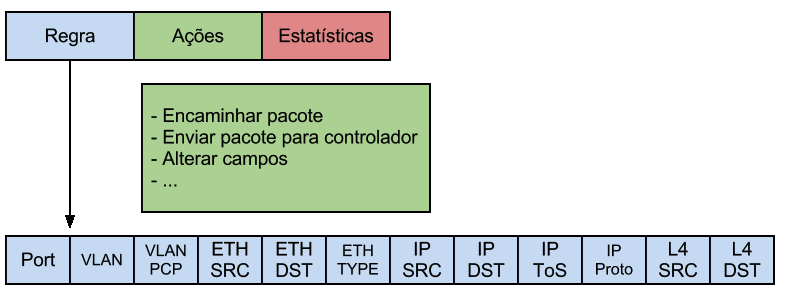
\includegraphics[width=110mm]{fluxoOpenflow.png} 
\caption{Exemplo de uma entrada na tabela de fluxos OpenFlow.} 
\label{fig:fluxoopenflow} 
\end{figure}

Esse pequeno conjunto de regras cria diversas possibilidades,
pois muitas das funcionalidades que são implementadas 
separadamente podem ser agrupadas em um único controlador
OpenFlow, utilizando um pequeno conjunto de regras. Alguns 
exemplos das possibilidades são apresentadas na \ref{fig:exemploSwitchOpenFlow}.
As entradas representam o uso do \textit{switch} OpenFlow
para realizar encaminhamento de pacotes na camada de enlace,
implementar um firewall e realizar encaminhamento de pacotes 
na camada de enlace utilizando VLANs, respectivamente.

\begin{figure}[hb] \centering
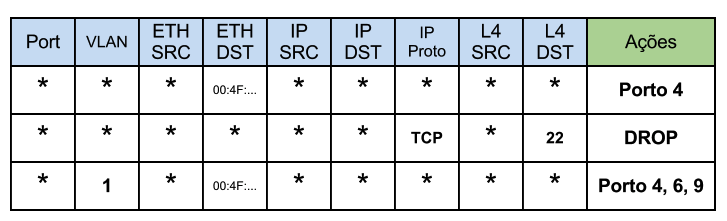
\includegraphics[width=110mm]{exemploSwitchOpenFlow.png} 
\caption{Exemplos de uso de um Switch OpenFlow.} 
\label{fig:exemploSwitchOpenFlow} 
\end{figure}

Apesar de possuir um conjunto pequeno de ações simples, 
alguns descrevem o OpenFlow como uma analogia ao conjunto 
de instruções de um microprocessador x86 que, apesar de 
pequeno e simples, provê uma vasta gama de possibilidades 
para o desenvolvimento de aplicações. O OpenFlow cria 
possibilidades semelhantes para o desenvolvimento de 
aplicações no contexto de redes de computadores. 

O \textit{OpenFlow} define um protocolo-padrão
para determinar as ações de encaminhamento de pacotes em
dispositivos de rede, como, por exemplo, comutadores,
roteadores e pontos de acesso sem fio. As regras e ações
instaladas no hardware de rede são responsabilidade de um
elemento externo, denominado controlador, que pode ser
implementado em um servidor comum, conforme Figura
\ref{fig:openflow}.

\begin{figure}[hb] \centering
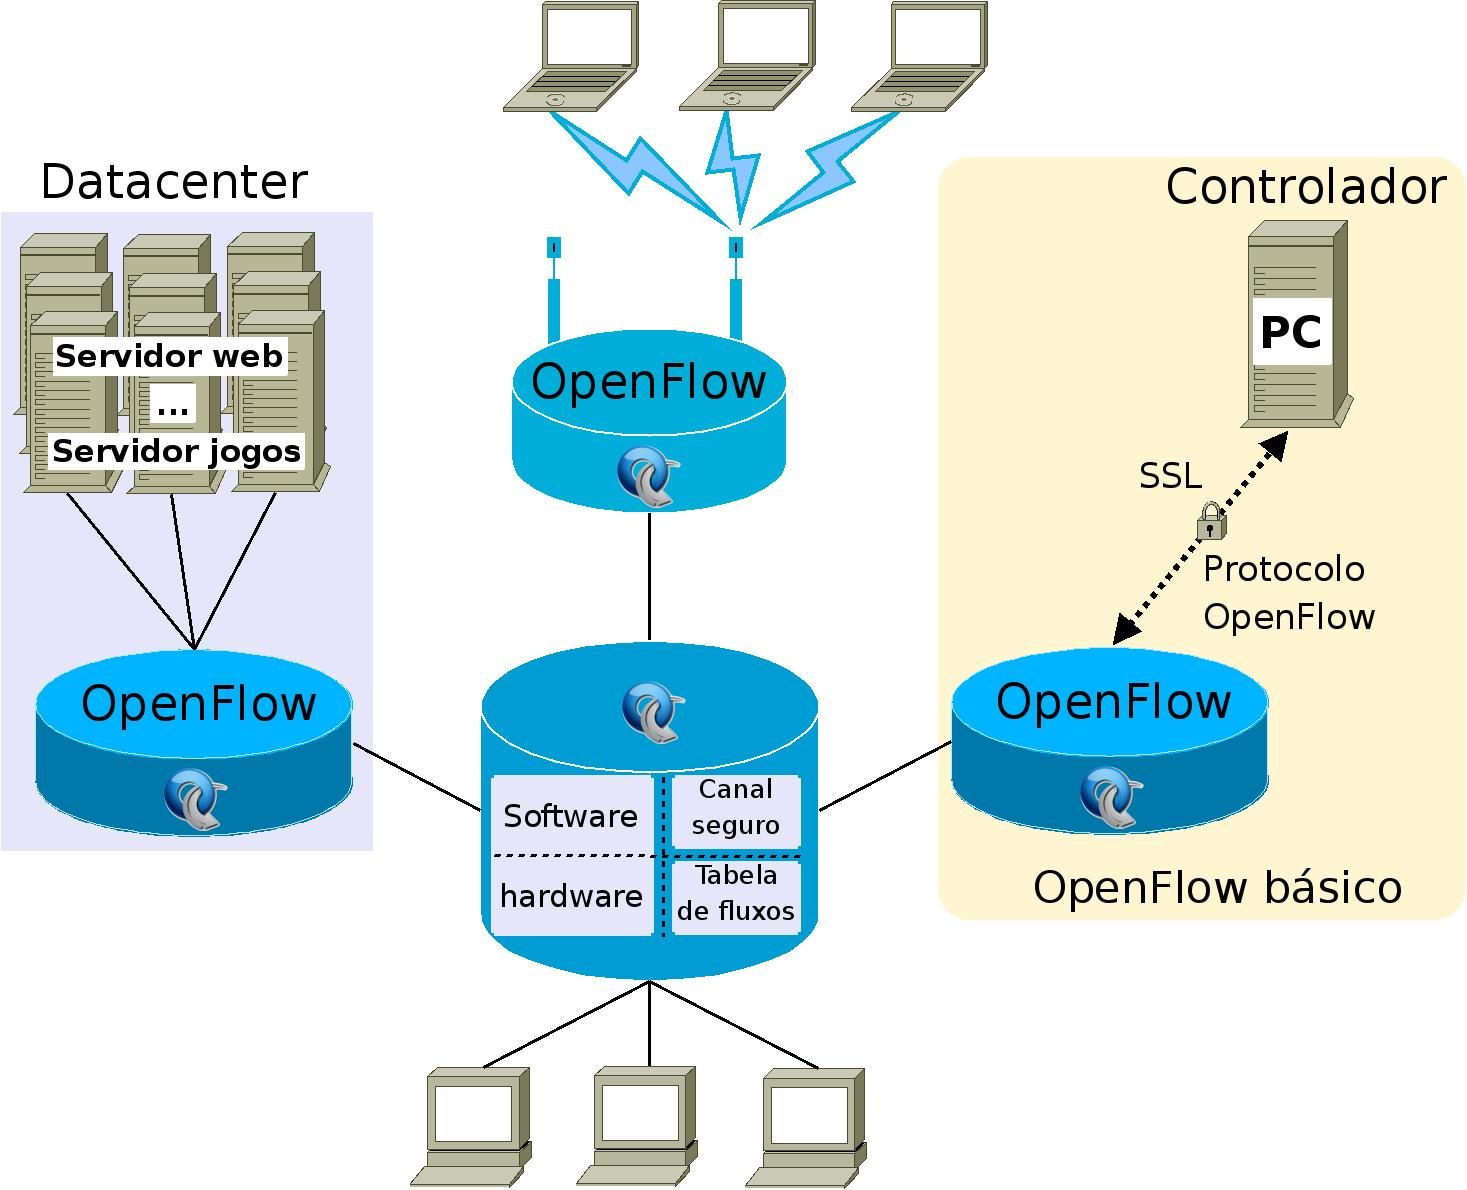
\includegraphics[width=110mm]{openflow.png} 
\caption{Rede com OpenFlow Habilitado} 
\label{fig:openflow} 
\end{figure}



\begin{figure}[hb] \centering
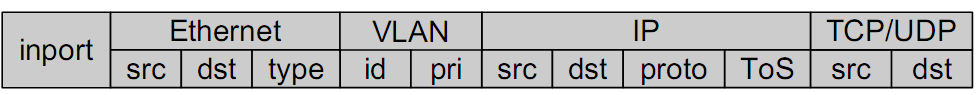
\includegraphics[width=160mm]{cabecalhoOpenflow.png}
\caption{Cabeçalho OpenFlow para a especificação dos fluxos}
\label{fig:cabecalhoOpenflow}
\end{figure}

De forma pragmática, a especificação \textit{OpenFlow}
(OPENFLOW, 2010) procura reutilizar as funcionalidades do
hardware existente (por exemplo, Access Control List – ACL
em switches e roteadores para implementar serviços como NAT,
firewall e VLANs) através da definição de um conjunto
simples de regras e das ações associadas: encaminhar,
descartar, enviar para o controlador, reescrever campos do
cabeçalho, etc.

\section{Introdução ao RouteFlow}

O RouteFlow é uma proposta de oferta de serviços de
roteamento IP remoto de forma centralizada, e que visa um
desacoplamento efetivo entre o plano de encaminhamento e o
plano de controle (ROUTEFLOW, 2011). O objetivo é tornar as
redes IP mais flexíveis pela facilidade de adição,
remoção e especialização de protocolos e algoritmos.
O RouteFlow armazena a lógica de
controle dos switches OpenFlow na infraestrutura de rede,
através de uma rede virtual composta por máquinas virtuais
(MV), cada uma executando um código
(engine) de roteamento de domínio público (open source).
Essas MVs podem ser interconectadas
de maneira a formar uma topologia lógica, espelhando a
topologia de uma rede física correspondente ou uma topologia
virtual simplificada. O ambiente virtual é armazenado em um
servidor externo, ou um conjunto deles, que se comunicam com
os equipamentos do plano de dados através de um controlador
OpenFlow, que transporta para o plano de encaminhamento as
decisões tomadas pelos protocolos de roteamento no plano de
controle (OSPF, BGP, RIP). A Figura
\ref{fig:visaoGeralRouteFlow} ilustra uma sub-rede com
switches programáveis, em que a lógica de roteamento é
implementada no servidor RouteFlow. O resultado consiste
numa solução flexível de alto desempenho e comercialmente
competitiva, a partir da combinação de recursos disponíveis,
como, por exemplo:

\begin{enumerate}[{a)}] 
\item switches programáveis de baixo
custo e software embarcado reduzido (OpenFlow); 
\item pilhas de protocolos de roteamento open source (QUAGGA, 2009; XORP,
2011); e 
\item servidor de prateleira de alto poder de
processamento e, também, de baixo custo. 
\end{enumerate}

Cabe ressaltar que, apesar de o controle estar fisicamente
centralizado, ele continua distribuído logicamente. Dessa
forma, não é necessária qualquer alteração dos protocolos de
roteamento existentes. Além disso, a solução pode tornar-se
mais escalável no futuro, com o uso
de vários servidores de alto desempenho.

\begin{figure}[hb] \centering
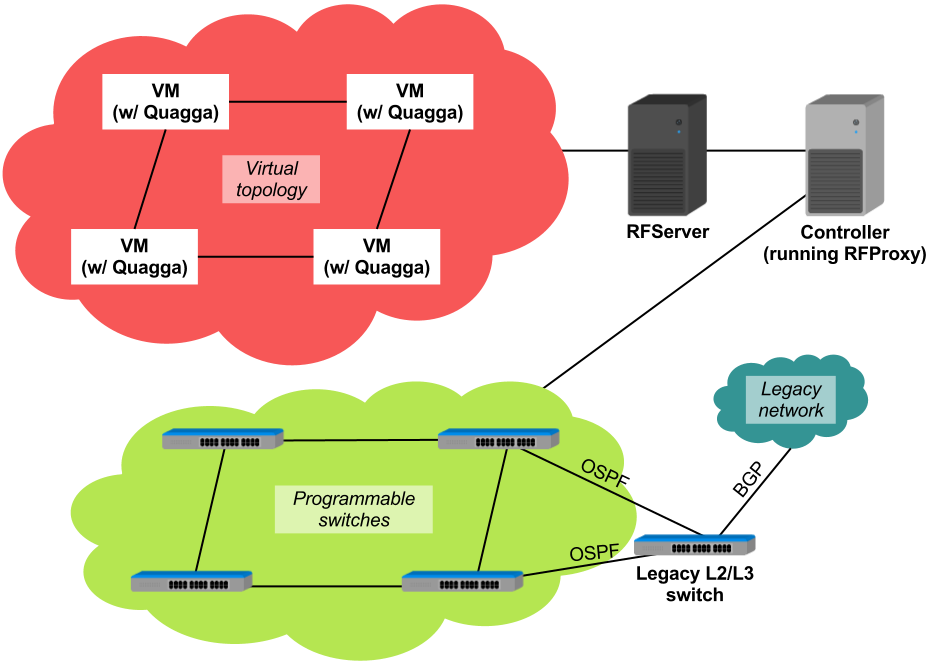
\includegraphics[width=135mm]{visaoGeralRouteFlow.png}
\caption{Visão geral do RouteFlow}
\label{fig:visaoGeralRouteFlow} 
\end{figure}

\section{Descrições dos Principais Componentes do RouteFlow}
O RouteFlow é dividido basicamente em três aplicações
básicas: RFClient, RFServer e RFProxy. Na Figura
\ref{fig:componentesRouteFlow} temos uma visão geral das
aplicações:

\begin{itemize} 
\item RFClient executa como um programa
executável em um máquina virtual, detectando
mudanças na tabela ARP do Linux e na tabela de roteamento.
As informações de roteamento são enviadas para o
RFServer quando são atualizadas.
\item RFServer é uma aplicação independente que gerencia as
máquinas virtuais que estão executando o RFClient. O
RFServer mantem o mapeamento entre as instâncias das
máquinas virtuais executando o RFClient e as interfaces
correspondentes aos switches e suas respectivas portas. É
conectado ao RFProxy para instruí-lo como configurar os
fluxos e também como configurar o Open vSwitch que mantém a
conectividade de todo o ambiente composto pelas máquinas virtuais.
\item RFProxy é uma aplicação responsável pelas interações
entre os switches OpenFlow (identificados pelos seus
datapaths) via o protocolo OpenFlow. Ele aguarda instruções
do RFServer e o notifica à respeito de eventos na rede.
Atualmente é executado como um módulo vinculado aos
controladores OpenFlow. O RouteFlow tem suporte aos
controladores NOX e POX, sendo que a proposta do trabalho é
adicionar suporte ao Floodlight. 
\end{itemize}

\begin{figure}[hb] 
\centering
\includegraphics[width=125mm]{componentesRouteFlow.png}
\caption{Componentes principais do RouteFlow}
\label{fig:componentesRouteFlow} 
\end{figure}

\section{Protocolo RouteFlow}

É o protocolo desenvolvido e usado para a comunicação entre
os componentes do RouteFlow. Nele, estão definidas as
mensagens e os comandos básicos para conexão e configuração
das máquinas virtuais e, também, gerenciamento das entradas
de roteamento em hardware. Entre os campos da
mensagem-padrão estão: identificação do controlador,
identificação da máquina virtual, tipo da mensagem,
comprimento e dados. O proxy RouteFlow recebe os comandos do
servidor RouteFlow através deste protocolo e de acordo com o
tipo de comando executa as principais ações, muitas delas
exigindo a comunicação com os switches físicos. A
comunicação com os switches físicos é feita via protocolo
OpenFlow, fazendo o proxy RouteFlow agir como
uma espécie de "tradutor" entre os dois protocolos.
\chapter{Proxy RouteFlow em Java}

\section{Introdução aos Proxies RouteFlow (RFProxy)}

Nos capítulo à respeito do projeto RouteFlow foi dado
uma visão geral de todos os três módulos usados para
construir o projeto. Esse capitulo se foca principal no 
módulo proxy, desenvolvido como foco principal do trabalho de
conclusão de curso.

Como já dito nos capítulos anteriores, o proxy RouteFlow ou
RFProxy atua como um tradutor de protocolos, convertendo
mensagens no protocolo RouteFlow para o protocolo OpenFlow
e vice-versa. Todos os eventos do ambiente físico são notificados
ao servidor na forma de mensagens, sendo as mesmas tratadas 
e processadas de acordo com o evento. Cada evento gera uma 
ação ao servidor (RFServer), que responde na forma de uma 
mensagem ao proxy (RFProxy), instruindo-o a tomar certa atitude.
Dentro dessas atitudes estão a criação das regras nos \textit{
switches OpenFlow}, fazendo toda a rede física se comportar
da maneira proposta pelo ambiente virtual e seus algoritmos de
roteamento.

As mensagens do protocolo RouteFlow, como já citado nos
capítulos anteriores, vem via o mecanismo de troca de mensagens
entre processos (IPC) implementado através do banco de dados
centralizado. Tal característica força o desenvolvedor escolher
as linguagens de programação com suporte à manipulação do
banco de dados usado pelo projeto RouteFlow, que no caso
é o MongoDB.

As mensagens do protocolo \textit{OpenFlow} são advindas do ambiente
físico e necessitam de algum mecanismo de captura e processamento.
Tal mecanismo é provido pelos softwares de controle \textit{
OpenFlow}. Dentre os diversos disponíveis, os mais famosos
são o NOX, o POX e o Floodlight. Todos os controladores
\textit{OpenFlow} são operados apenas como 
interfaces de programação, provendo todas as funções de captura
de eventos e criação de mensagens do protocolo \textit{OpenFlow}.

Cada um dos controladores citados acima foi desenvolvido em
uma linguagem de programação diferente, forçando o desenvolvedor
a trabalhar na mesma linguagem do controlador de forma a 
opera-lo como forma de interface de programação (API). 
Cada controlador possui vantagens exclusivas, tendo sido construídos
com propósitos diferentes. O controlador NOX se destaca pela
performance, pelo fato de ser construído em C++ e possui
código compilado. O controlador POX se destaca pela
facilidade de programação provida pela linguagem Python mas
possui desempenho inferior devido ao fato do Python ser
interpretado. 

O controlador escolhido para uso neste trabalho foi 
o Floodlight. Sendo desenvolvido para ser usado
principalmente por  administradores de rede, possui uma 
série de aplicações nativas que permitem o seu controle
via aplicações externas. Uma dessas aplicações nativas 
permite a recepção de mensagens via mensagens REST,
possibilitando ao desenvolvedor manipular sua rede sem
a necessidade de programar um módulo dedicado. Tal fato
dificultou o desenvolvimento do trabalho, visto que grande 
parte da documentação disponível para consulta era voltada
apenas para os administradores, sem levar em consideração os 
desenvolvedores de aplicações em Java. O fato
de ter sido construído em Java pode impactar em seus desempenho
mas tal impacto é recompensado visto o grande número de 
recursos disponíveis. Um dos recursos que pode ser citado
é a interface gráfica usada para visualização da rede que
no futuro poderá ser adaptada para uso como o projeto 
RouteFlow. A comunidade de usuários é grande e bastante
ativa, fato notado pela grande quantidade de postagens no
fórum oficial do controlador.

Os dois proxies RouteFlow (RFProxy) já existentes durante a 
criação desse trabalho seguem um mesmo algoritmo, o que 
facilita muito o entendimento geral. A maior dificuldade no
desenvolvimento de um novo proxy RouteFlow (RFProxy) são
as características exclusivas de cada linguagem de programação,
cabendo ao desenvolvedor as adaptações necessários para 
implementar o algoritmo. A linguagem Java já possuía uma
ótima API para comunicação com o banco de dados MongoDB
e para a manipulação de mensagens no protocolo JSON. Um fato
que trouxe certa dificuldade no trabalho foi o desenvolvimento
de uma aplicação com múltiplas threads em Java. 

A Figura \ref{fig:esquematicoProxy} ilustra de forma simples as
funções básicas bem como a direção das informações tratadas
pelo proxy RouteFlow (RFProxy). É interessante notar que o 
proxy só se comunica com com o restante do ambiente através
do mecanismo de troca mensagens entre processos (IPC) basedo
no banco de dados centralizado.
\newline
\newline
\newline
\newline


\begin{figure}[h] 
\centering
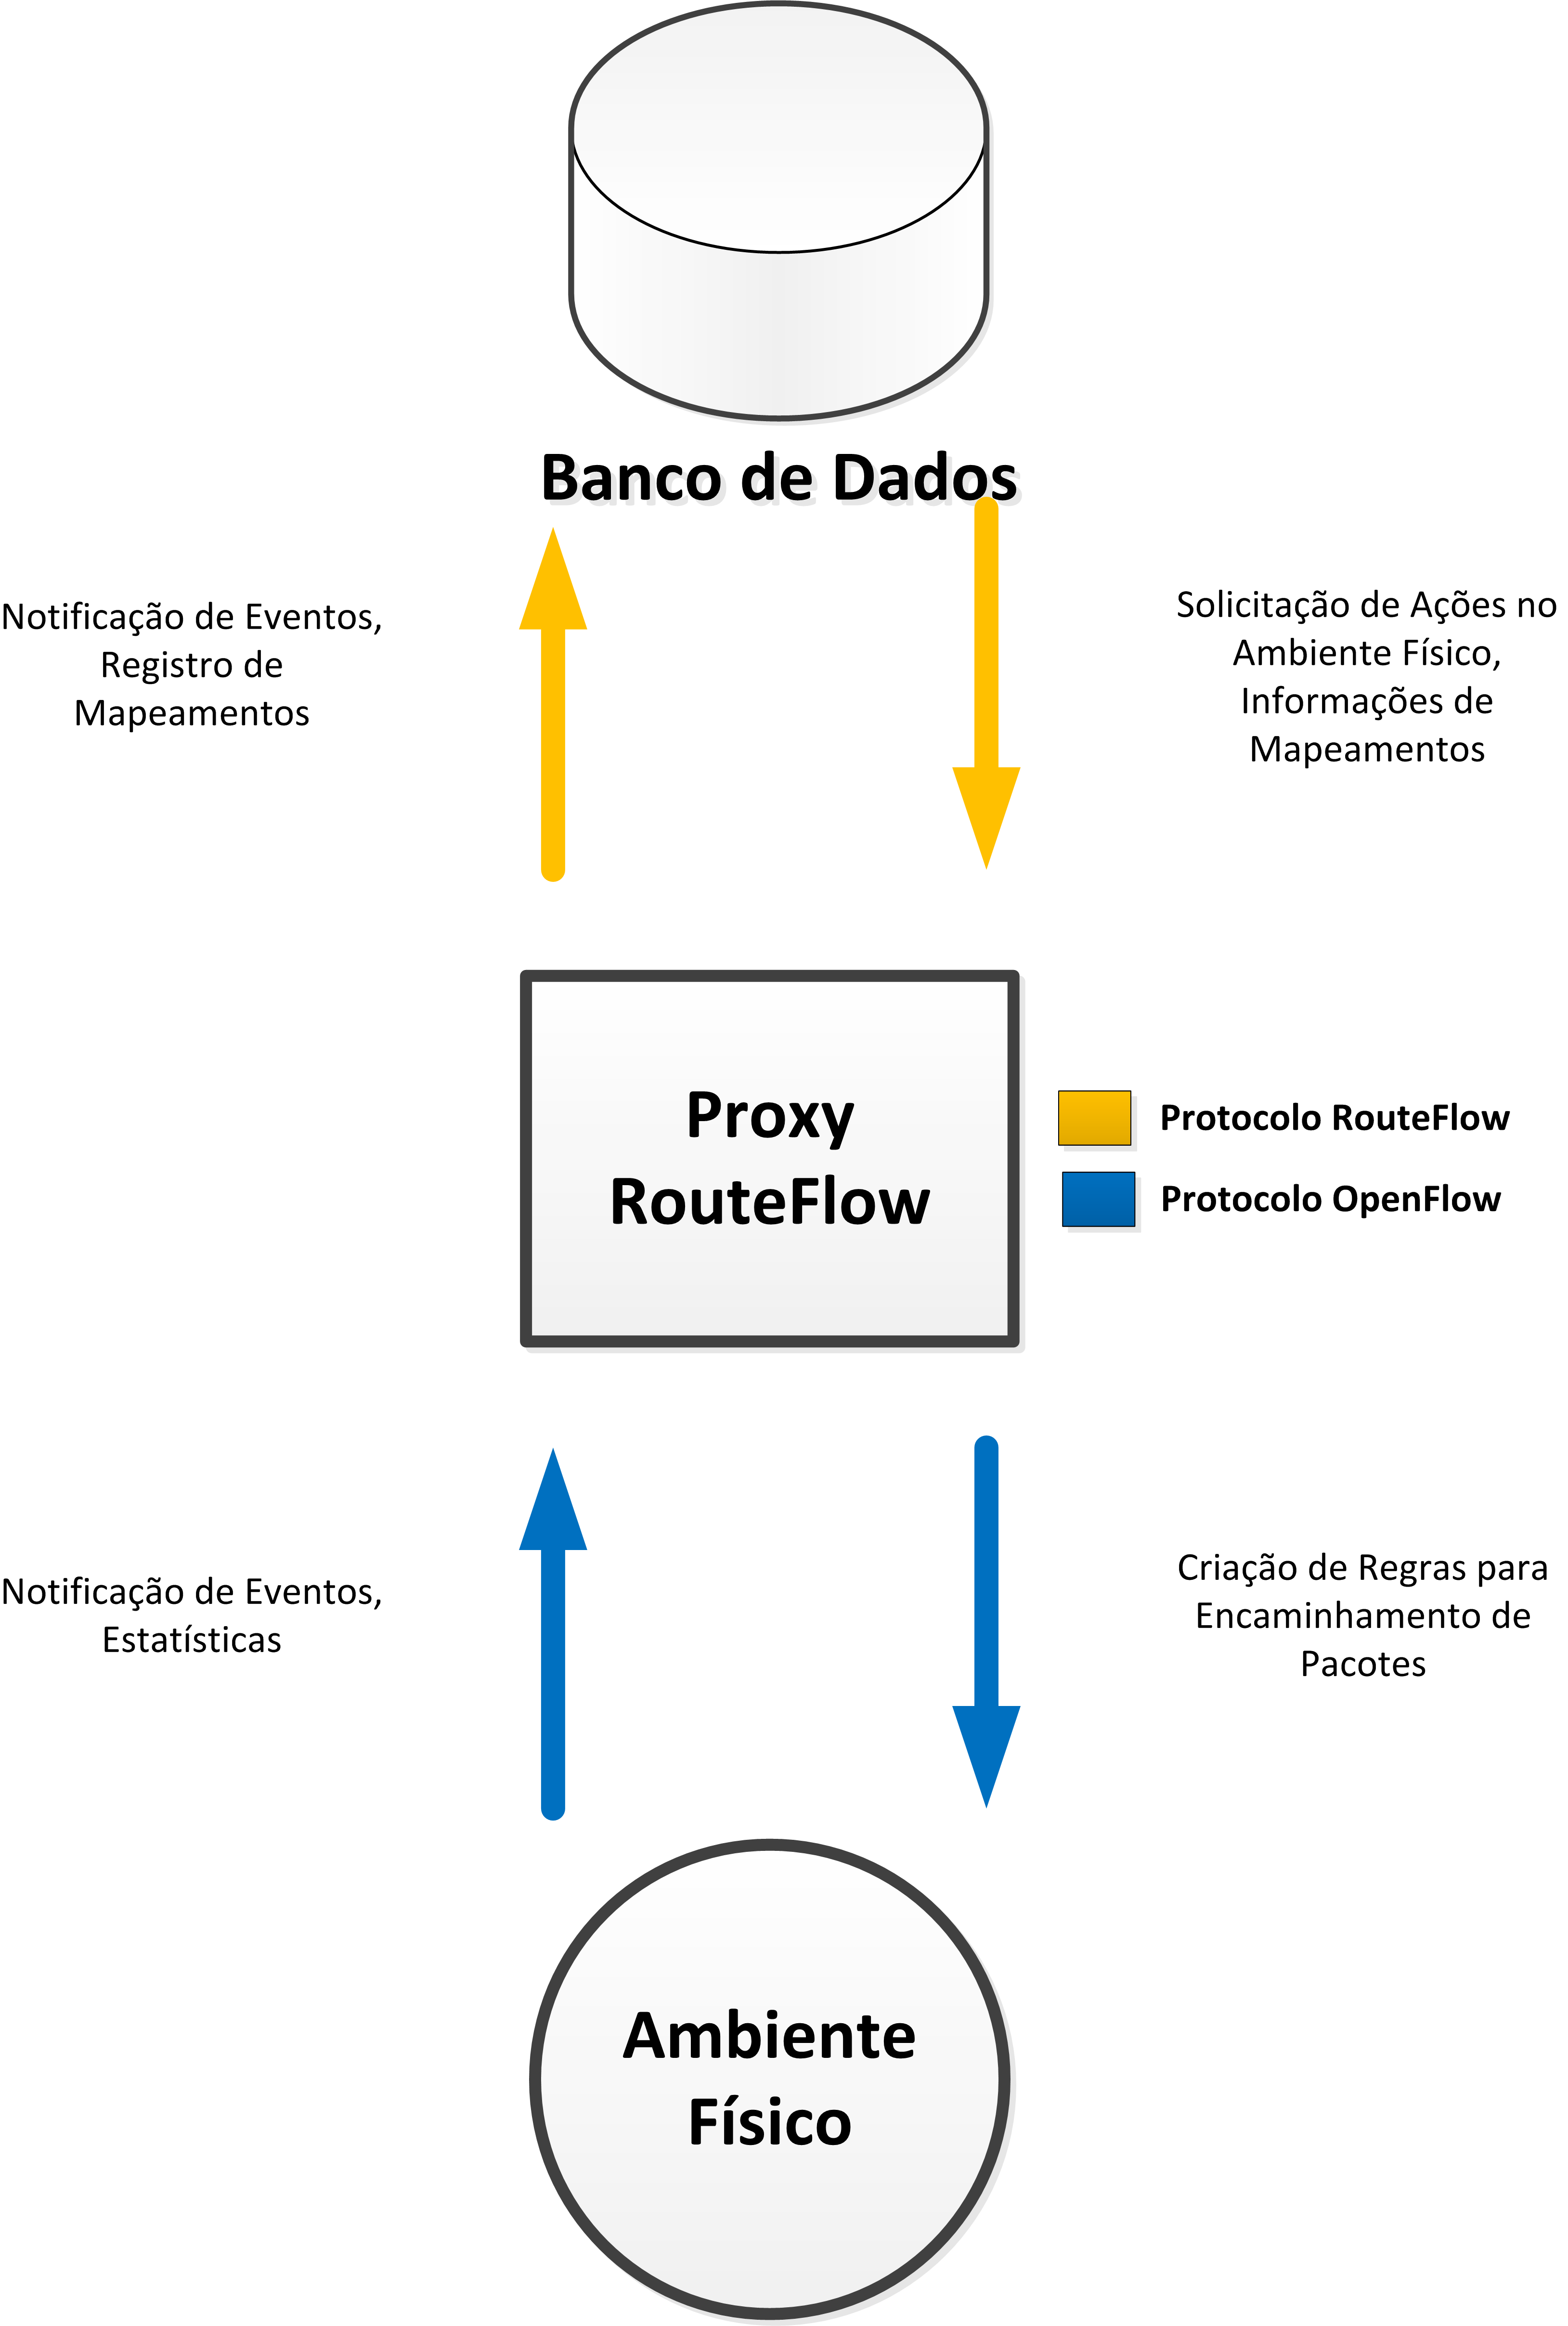
\includegraphics[width=120mm]{esquematico_geral_proxy.png}
\caption{Esquema Geral do Proxy RouteFlow (RFProxy).}
\label{fig:esquematicoProxy} 
\end{figure}
 

\section{Descrição Geral da Estrutura do Proxy RouteFlow em Java}

Todos os componentes do proxy RouteFlow em Java foram agrupados em classes. O agrupamento em classes 
facilita a 
organização geral do código bem como a sua futura manutenção. Abaixo temos os componentes do proxy com 
suas respecitivas descrições:

\begin{itemize}
\item \textit{MongoIPCMessageService:} Responsável pela
 comunicação entre o servidor RouteFlow e o proxy 
RouteFlow. A arquitetura básica do projeto RouteFlow 
faz uso de um banco de dados não SQL para troca de 
mensagens entre seus componentes, sendo que o banco 
de dados escolhido foi o MongoDB. 

O MongoDB possui 
alto desempenho sendo totalmente escrito em C++, outro
 aspecto importante é o fato de não ser SQL, o 
que facilita a sua integração com as  principais linguagens
 de programação. 
O RouteFlow cria inúmeras tabelas no banco de dados, cada uma 
responsável pela comunicação entre um par 
de componentes, como toda comunicação é feita através de um 
sistema de banco de dados é possível que a 
comunicação entre componentes seja feita de forma simples, sem 
nenhum vinculo com a linguagem de 
implementação do mesmo. 

O componente MongoIPCMessageService 
cria um IPC (Inter-Process Communication) 
entre o servidor RouteFlow e o proxy RouteFlow. Os comandos são 
enviados de um componente para o outro 
na forma de mensagens pré-definidas. Cada mensagem define uma 
ação à ser tomada em relação aos eventos 
que vão ocorrendo ao longo da execução do ambiente. No corpo da 
mensagem estão os parâmetros que 
deverão ser usados para tomada da ação. Todas as mensagens que 
são colocadas na tabela pelo servidor RouteFlow 
possuem um campo que indica se a mesma já foi tratada e em caso 
negativo cabe ao proxy tomar a ação e 
atualizar o campo da mensagem. Para tratamento das mensagens é 
gerado uma thread em looping infinito 
cujo único proposito de existência é o tratamento de novas mensagens. 
Essa característica pretende ser melhorada nas próximas versões 
do RouteFlow;
\item \textit{RFProtocolFactory:} Responsável pela criação das 
mensagens do protocolo RouteFlow. Cada 
tipo de mensagem RouteFlow é representada por um código e 
por uma respectiva classe. É papel do 
RFProtocolFactory retornar os objetos de mensagens à partir de 
seu código. Esta estrutura facilita a 
inserção de novas mensagens no ambiente evitando a reprogramação 
de outras classes;
\item \textit{RFProtocolProcessor:} Responsável pelo processamento 
de mensagens vindas do servidor 
RouteFlow. Este componente define o como será tratada cada mensagem 
vinda do servidor RouteFlow. As 
mensagens são lidas através do IPC e repassadas para tratamento.
\item \textit{AssociationTable:} Tabela mantida pelo proxy para armazenar 
a associação entre portas no 
ambiente virtual e porta no ambiente físico.
\end{itemize} 

\section{Descrição das Mensagens Traduzidas pelo Proxy RouteFlow}

\begin{itemize}
\item \textit{PortRegister}
\item \textit{PortConfig}
\item \textit{DatapathConfig}
\item \textit{RouteInfo}
\item \textit{FlowMod:} Mensagem utilizada para 
solicitação da instalação de regras nos switches 
OpenFlow. As mensagens FlowMod possuem em seu 
corpo um conjunto de parâmetros que define uma nova regra 
a ser aplicada à um switch OpenFlow. Cabe ao proxy 
criar a regra e envia-la corretamente ao switch. 
Para envio das regras é necessário a manipulação do 
protocolo OpenFlow. O Floodlight fornece uma série de 
funções para esse proposito, sendo usado como uma 
API de comunicação entre os switches OpenFlow e o 
proxy.
\item \textit{DatapathPortRegister:} Mensagem utilizada 
para registrar as portas dos switches OpenFlow 
no servidor RouteFlow. Esse registro é feito para que cada 
porta seja associada à uma porta da máquina 
virtual do ambiente virtual.
\item \textit{DatapathDown:} Mensagem utilizada para que 
o proxy informe ao servidor RouteFlow sobre a 
desconexão de um switch OpenFlow. O Floodlight, no papel 
de controlador OpenFlow, mantem um conjunto de 
informações à respeito dos switches OpenFlow ativos, 
podendo detectar quedas nas conexões dos mesmos. O 
servidor RouteFlow necessita ter esse tipo de informação para 
possíveis alterações nas regras dos 
switches OpenFlow.
\item \textit{VirtualPlaneMap:} Mensagem utilizada para que 
o proxy associa cada porta do switch 
OpenFlow à uma porta de uma máquina virtual no ambiente 
virtual.
\item \textit{DataPlaneMap:} Mensagem utilizada para que o 
servidor RouteFlow informe ao proxy à 
respeito de uma associação de porta bem sucedida. O proxy 
mantém uma tabela de associação entre portas 
no ambiente virtual e portas no ambiente físico.
\end{itemize}


\chapter{Resultados}

%\section{Principais Benefcios do Uso do Controlador Floodlight}


\chapter{Conclusão}

\section{Trabalhos Futuros}

Como principal trabalho futuro estará a manutenção e 
inserção de novas funcionalidades no proxy RouteFlow.
Durante o desenvolvimento desse trabalho o Projeto
 RouteFlow ganhou suporte ao uso simultâneo de proxies, 
permitindo que cada trecho da rede seja controlado por um
proxy diferente. Tal funcionalidade exige a inserção de 
mais alguns parâmetros no código original desenvolvido
 durante o trabalho, sendo assim o próximo trabalho futuro.

Outro trabalho futuro será a remoção do looping infinito 
para leitura de mensagens vindas do servidor RouteFlow, 
um dos pesquisadores do Projeto RouteFlow está
desenvolvendo um mecanismo de comunicação mais ágil e
 eficaz. Esse mecanismo também deverá ser portado ao 
 novo proxy de forma a sempre se manter atualizado.

\chapter{Agradecimentos}

\begin{itemize}
\item Allan Vidal -- CPqD, Campinas - SP
\item Cesar Augusto Cavalheiro Marcondes -- UFSCar, 
São Carlos - SP
\item Christian Esteve Rothenberg -- CPqD, Campinas - SP
\item Eder Leão Fernandes -- CPqD, Campinas - SP
\item Jorge Henrique de Barros Assumpção -- CPqD, Campinas - SP
\item Marcos Rogerio Salvador -- CPqD, Campinas - SP
\item Sachin Sharma -- Ghent, Bélgica
\item Toda a equipe do Forum do Floodlight
\end{itemize}

\bibliographystyle{abnt}
\nocite{*}
\bibliography{bare_conf}

\end{document}
